\section{DESCRIPCION DE LA EMPRESA} 

Plaza Vea es una cadena de supermercados que forma parte del conglomerado peruano Intercorp, el cual también integra a los supermercados Vivanda.

			\begin{figure}[htb]
				\begin{center}
					
\includegraphics[width=10cm]{./Imagenes/3}
				\end{center}
			\end{figure}

	\begin{itemize}
   	 \item Plaza Vea es la marca de hipermercados y supermercados de la empresa Supermercados Peruanos S.A. perteneciente al prestigioso Grupo Interbank.
	\item	Es una empresa 100 por ciento peruana que da trabajo a más de 10 mil personas en Lima y provincia, distribuidas entre sus más de 80 tiendas, ¡Y seguimos creciendo!
	\item	Fue el primer hipermercado en salir a provincias en el año 2007 lo que nos valió una serie de reconocimientos como el Gran Premio a la Creatividad Empresarial y un Effie de Plata.
	\item	En el 2009 fue elegido como una de las mejores empresas para trabajar en el Perú, ocupamos el puesto 7 en el ranking general de Great Place to work.
	\item	En el 2009 Plaza Vea logra certificación internacional para sus alimentos frescos, es la primera cadena de supermercados del país con certificación HACCP.
	\item	Plaza Vea sigue creciendo por todo el país y se sigue extendiendo.

    
 	 \end{itemize}

MISION:
Somos una empresa peruana de venta de productos al por menor, tanto en perecibles como en abarrotes pasando por textil y electro que basa su desarrollo y crecimiento en una sólida cultura de servicio que busca generar excelentes experiencias de compra para nuestros clientes. Crear excelentes experiencias de compra para que nuestros clientes regresen y tengan una mejor calidad de vida.

VISION:
Ser la primera opción de compra para todos los peruanos siendo Honestos, cuidadosos y ordenado, ser serviciales, muy trabajadores; trabajando en equipo con la búsqueda de un ideal común que nos una con esfuerzo y dedicación, ofreciendo productos de calidad gracias a una capacidad de innovación sostenible en el tiempo. 

\subsection{ ORGANIZACION  DE LA EMPRESA - PLAZA VEA}

Plaza Vea, cuenta con mas 58 locales, logrando de esta manera ser el pilar de la expansión de las operaciones de la empresa tanto en su formato de hipermercado como el de supermercado.

				\begin{figure}[htb]
				\begin{center}
					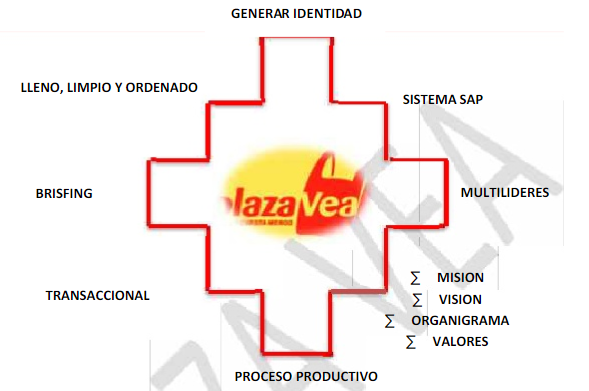
\includegraphics[width=15cm]{./Imagenes/4}
				\end{center}
			\end{figure}



\begin{enumerate}[a)]
        \item Organigrama de la Empresa

			\begin{figure}[htb]
				\begin{center}
					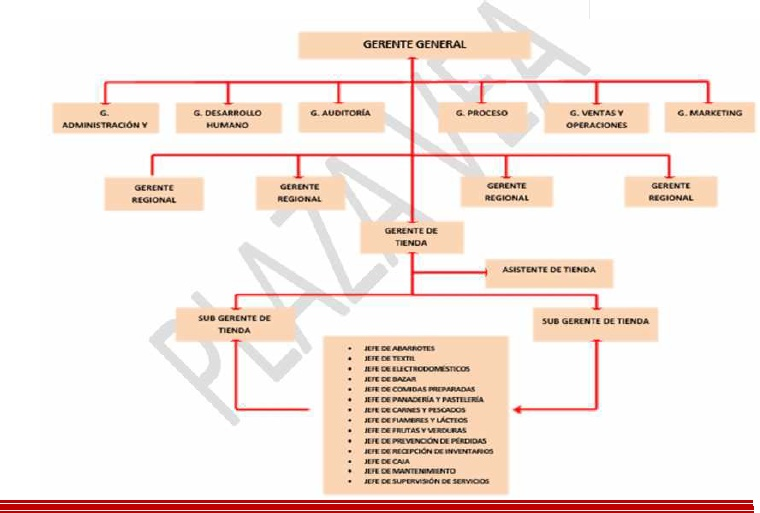
\includegraphics[width=15cm]{./Imagenes/5}
				\end{center}
			\end{figure}
        \item Cadena de Valores

			\begin{figure}[htb]
				\begin{center}
					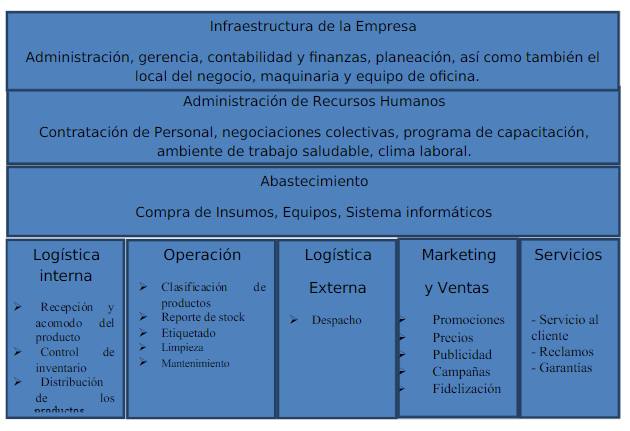
\includegraphics[width=15cm]{./Imagenes/6}
				\end{center}
			\end{figure}

	\item FODA

			\begin{figure}[htb]
				\begin{center}
					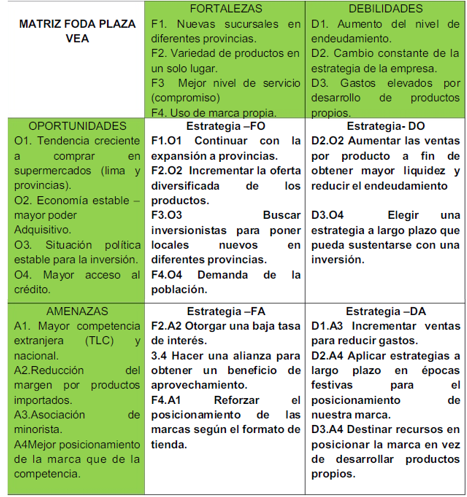
\includegraphics[width=15cm]{./Imagenes/7}
				\end{center}
			\end{figure}

	\item OBJETIVOS ESTRATÉGICOS DE LA EMPRESA PLAZA VEA

		\begin{itemize}
  		  \item[$*$] Capacitar al personal para que este en sintonía con la vocación de servicio y con propósitos de exceder expectativas del cliente.
		\item[$*$] Se la solución diaria y semanal preferida para los consumidores.
		\item[$*$ ]Estar siempre a la Vanguardia; siempre estar en campañas promocionales.
		\item[$*$] Brindar una buena Infraestructura, Comodidad, Seguridad y centros de esparcimiento en nuestras instalaciones.

		\item[$*$] Mantener precios competitivos.
		\item[$*$] Ofrecer un catálogo de productor didácticos en la Web.
		\item[$*$] Promocionar e incentivar la compra electrónica entre ciudadanos peruanos y personas que radican en el extranjero
		\item[$*$] Acaparar nuevos nichos de mercado.
		\item[$*$] Incursionar con más mercados en provincia.
		\item[$*$] Implementación de Data WereHouse
		\item[$*$] Mantener o mejorar la imagen de la empresa.


		\end{itemize}

	\item OBJETIVOS DE ORGANIZACIÓN (APRENDIZAJE E INNOVACIÓN) DE PLAZA VEA

		\begin{enumerate}[1.]
  			  \item Competencias. - dentro de los factores que se han identificado, podemos establecer los
siguientes objetivos:
			\begin{itemize}
  			  \item[$*$] Capacitación para los siguientes factores:

				\begin{itemize}

  				  \item Nivel Profesional adecuado
				  \item Adecuados niveles de productividad
				  \item Baja capacitación en tecnologías de la información
				  \item Personal con poca experiencia técnica
				 \item Bajos niveles de capacitación

				\end{itemize}

			 \item[$*$] Coaching (desarrollo de aptitudes para el liderazgo para mejorar los siguientes aspectos

				\begin{itemize}

  				  \item Alta efectividad en la delegación de funciones
				  \item Alta mayores canales de comunicación

				\end{itemize}

			 \item[$*$] Establecer una relación laboral adecuado para poder tener un manejo adecuado de las relaciones:

				\begin{itemize}

  				  \item Estabilidad laboral
				  \item Limitaciones para atraer gente altamente creativa

				\end{itemize}


			\end{itemize}

  			  \item Clima laboral. - dentro de este aspecto, podemos mencionar los siguientes objetivos:

				\begin{itemize}

				\item[$*$] Crear un clima organizacional adecuado objetivo que busca manejar los efectos del siguiente factor:

				\begin{itemize}

  				  \item Clima organizacional adecuado

				\end{itemize}


				\item[$*$] Cambiar cultura organizacional para manejar adecuadamente los siguientes factores:

				\begin{itemize}

  				  \item Cultura de valores, principios
				  \item Identificación con la empresa

				\end{itemize}


			\end{itemize}
    
		\end{enumerate}

	\item OBJETIVOS INTERNOS DE LA EMPRESA PLAZA VEA

	Los factores que afectan los procesos internos de la empresa han generado los siguientes objetivos:
		\begin{enumerate}[1.]

    		\item Proceso de Innovación. - bajo este proceso se han definido los siguientes objetivos que buscan manejar el efecto de los factores que inciden sobre dichos procesos:

			\begin{itemize}

				\item[$*$] Identificar mercados potenciales, para manejar los factores siguientes:

				\begin{itemize}

  				  \item Empresas interesadas en el sector
				\item Ingreso al Mercado de Lima
				\item Ubicación cercana de mercados potenciales
				\item Adecuadas vías de comunicación
				\item Plan de integración Perú – Ecuador
				\item Sinergia del sistema de Cajas Municipales

				\end{itemize}


				\item[$*$] Crear productos / ofertar nuevos servicios, objetivos que incide sobre los siguientes factores:

				\begin{itemize}

  				  \item Inversión Pública
				\item Privatizaciones
				\item Recuperación del PBI
				\item Condiciones de Libre Mercado
				\item Promoción del Estado a las PYMES
				\item Niveles de desempleo y subempleo
				\item Promoción del Banco Agropecuario
				\item Normas tributarias del sector 


				\end{itemize}

			\end{itemize}

   		\item Procesos de Operaciones. - los procesos de operaciones se establecen con la finalidad de
buscar la eficiencia en lo que hacemos para brindar nuestros productos. Dentro de estos
procesos se han definido los siguientes objetivos:


			\begin{itemize}

				\item[$*$] Mejorar niveles de productividad

				\begin{itemize}

  				  \item Nivel adecuado de tecnificación interna
				\item Desarrollo tecnológico mundial
				\item Intercambio técnico por la globalización
				\item Desarrollo tecnológico de la competencia
				\item Orientación empresarial


				\end{itemize}


				\item[$*$] Minimizar el efecto de factores políticos.

				\begin{itemize}

  				  \item Débil estabilidad jurídica
				\item Débil estabilidad política
				\item Injerencia política
				\item Normas de austeridad y contratación del Estado


				\end{itemize}
				\end{itemize}


   		\item Procesos de comercialización.- Para manejar un valor más adecuado de los productos o
servicios que ofrecemos, se definen los siguientes objetivos: 

				\begin{itemize}

				\item[$*$] Incrementar participación de mercado

				\begin{itemize}

  				  \item Participación de mercado
				\item Retiro de bancos comerciales de provincias
				\item Poco acceso a organismos privados y públicos
				\item Zona geográfica con clima inestable

				\end{itemize}

				\end{itemize}


    
		\end{enumerate}

	\item OBJETIVOS DEL CLIENTE DE LA EMPRESA PLAZA VEA

		\begin{itemize}

				\item[$*$] Atributos.- dentro de este concepto podemos establecer los siguientes objetivos estratégicos:

				\begin{itemize}

  				  \item Mantener Precios Competitivos
				\item Tasas de interés competitivas
				\item Mejorar constantemente la Calidad del Producto
				\item Producto exclusivo y de calidad
				\item Diversificar los productos que ofrece la CMAC
				\item Falta mayor diversificación de productos


				\end{itemize}


				\item[$*$] Imagen.- los objetivos definidos para el caso del atributo de imagen dentro de la perspectiva de cliente son los siguientes:
				\begin{itemize}

  				  \item Proyectar imagen de solidez y confianza
				\item Limitada infraestructura

				\end{itemize}

				\item[$*$] Relaciones con el cliente.- Se han establecido los siguientes objetivos:

				\begin{itemize}

  				  \item Establecer un Programa de CRM (Customer Relationship Management)
				\item Lealtad y satisfacción del cliente
				\item Promoción y formalización de negocios
				\item Falta programa de administración de clientes

				\end{itemize}

		\end{itemize}

	\item OBJETIVOS FINANCIEROS DE LA EMPRESA PLAZA VEA
		
	Dentro de la perspectiva financiera tenemos los siguientes objetivos:

			\begin{itemize}

  				  \item Incrementar el valor patrimonial, dentro de este objetivo se enmarcan los siguientes factores:
				\item Crecimiento sostenido
				\item Rentabilidad adecuada
				\item Capacidad de Endeudamiento
				\item Reducir costos operativos, este objetivo busca manejar los siguientes factores:
				\item Limitados fondos internos
				\item No existe metodología de costeo eficaz
				\item Diversifica fuentes de financiamiento, para manejar una adecuada estructura financiera:
				\item Líneas de financiamiento externas para microfinanzas
				\item Reducir efecto de factores externos, para minimizar los efectos de:
				\item Nivel de la inflación
				\item Incremento de la devaluación
				\item Percepción de riesgo país


			\end{itemize}

	\item MAPA ESTRATEGICO DE LA EMPRESA PLAZA VEA


	Para el Desarrollo del Mapa Estratégico y Balanced ScoreCard de la Empresa Plaza Vea, se utilizó el software de Reportes Tableau.
Tableau es un software de análisis de datos con una excelente capa de visualización y presentación, considerado por muchos como uno de los mejores programas para la presentación visual de datos y con muy alta clasificación en la facilidad de uso, por lo que sigue muy de cerca a Microsoft Excel.

			\begin{figure}[htb]
				\begin{center}
					
\includegraphics[width=10cm]{./Imagenes/8}
				\end{center}
			\end{figure}


			\begin{figure}[htb]
				\begin{center}
					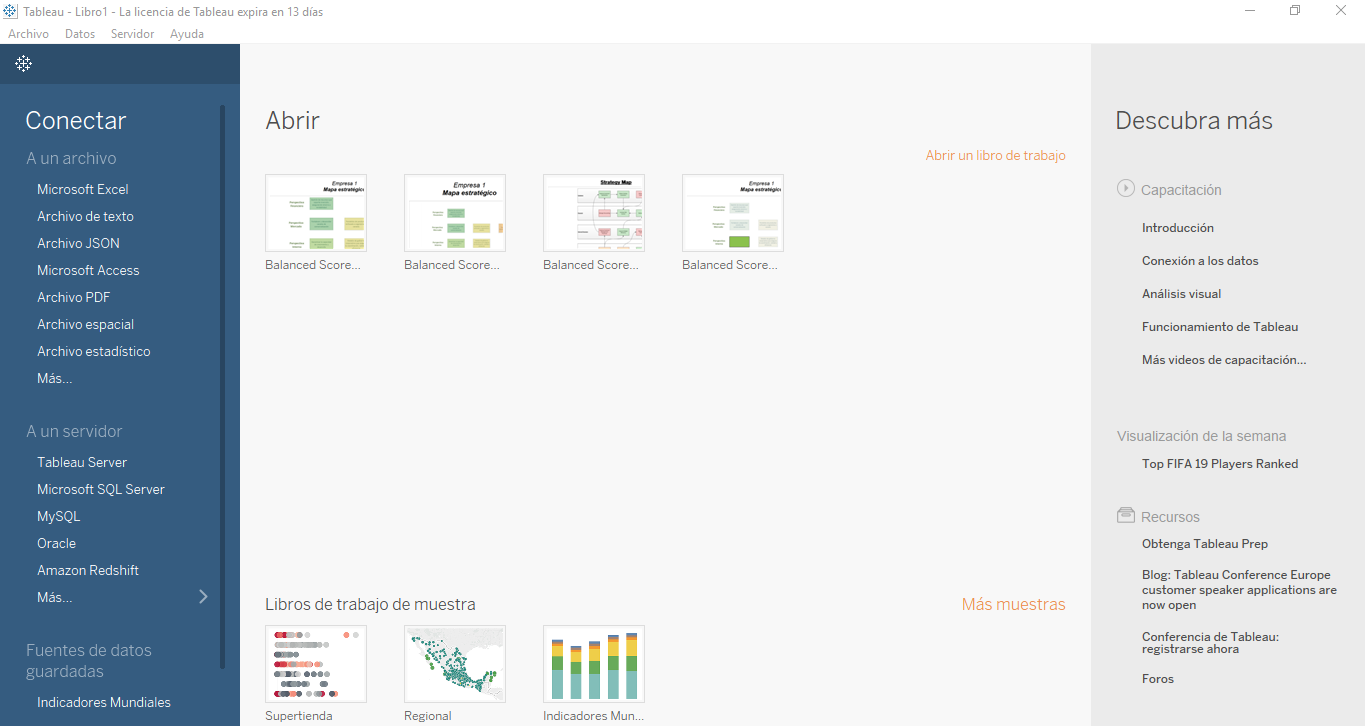
\includegraphics[width=17cm]{./Imagenes/9}
				\end{center}
			\end{figure}


			\begin{figure}[htb]
				\begin{center}
					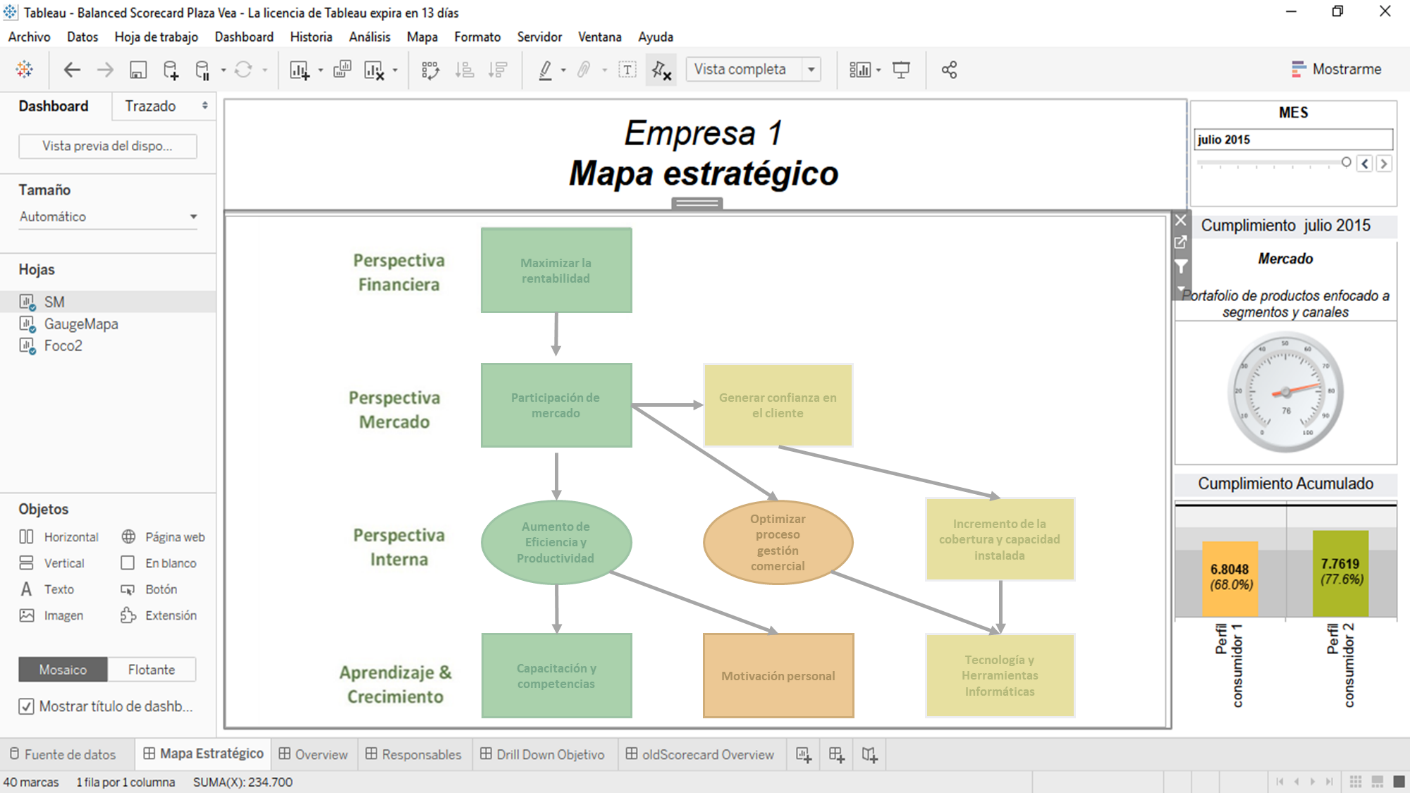
\includegraphics[width=17cm]{./Imagenes/10}
				\end{center}
			\end{figure}


			\begin{figure}[htb]
				\begin{center}
					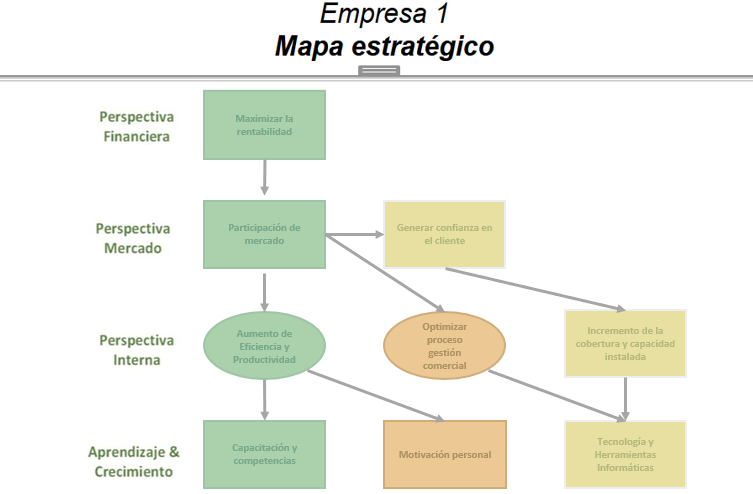
\includegraphics[width=17cm]{./Imagenes/11}
				\end{center}
			\end{figure}

	\item BALANCED SCORECARD DE LA EMPRESA PLAZA VEA

			\begin{figure}[htb]
				\begin{center}
					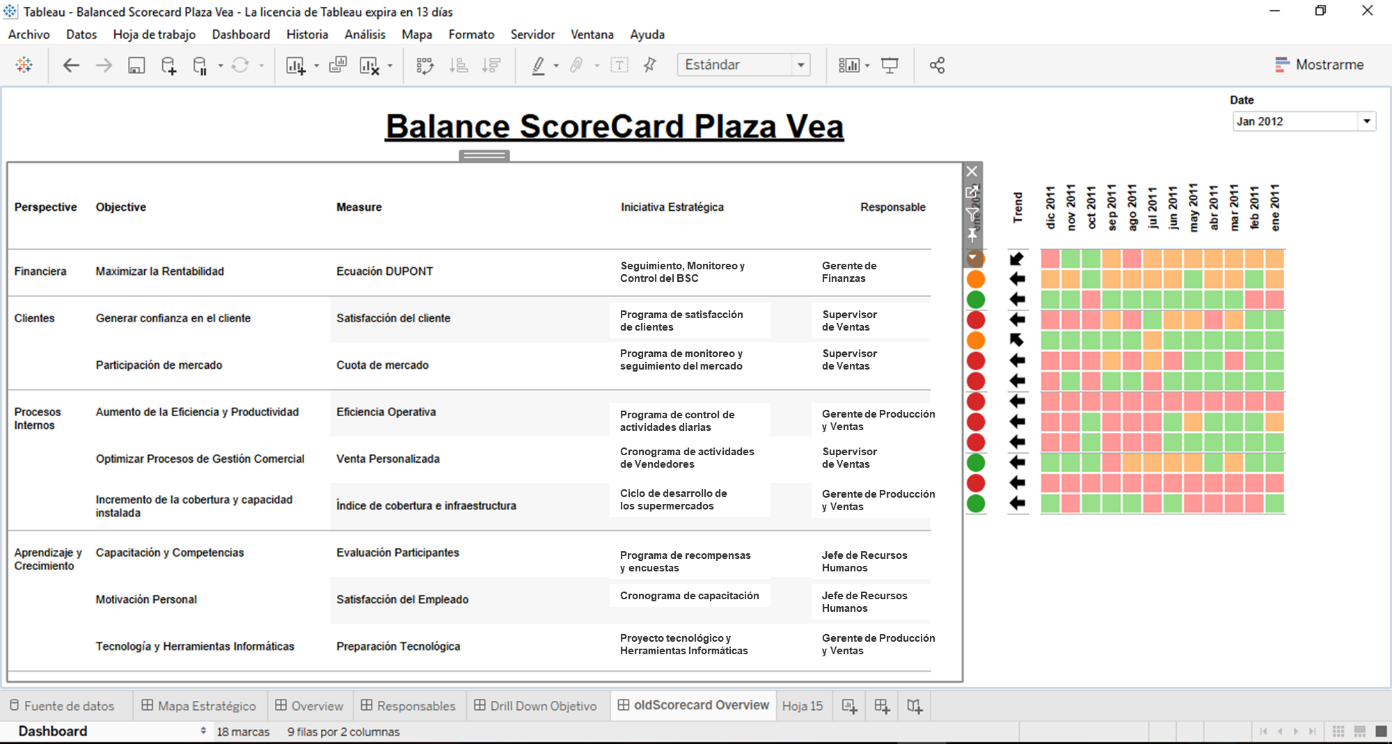
\includegraphics[width=17cm]{./Imagenes/12}
				\end{center}
			\end{figure}

			\begin{figure}[htb]
				\begin{center}
					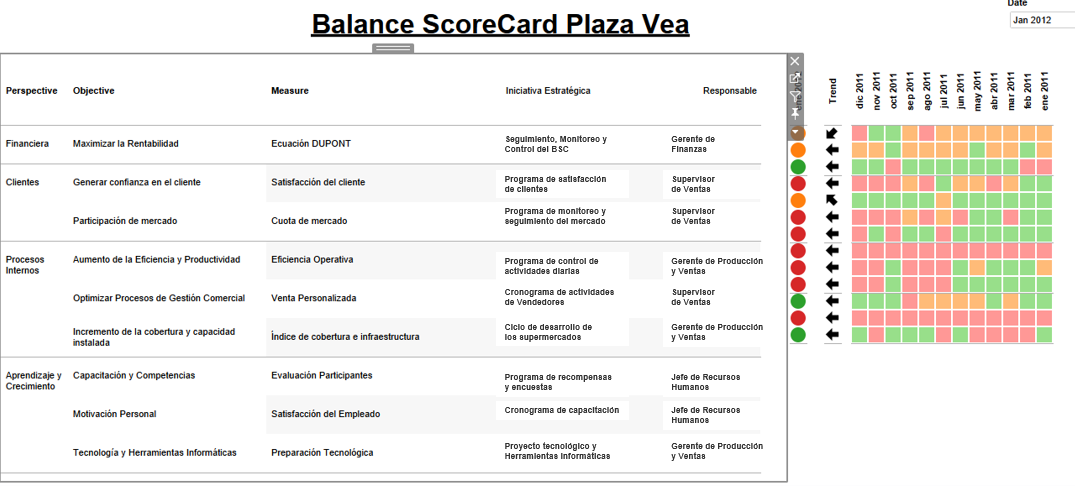
\includegraphics[width=17cm]{./Imagenes/13}
				\end{center}
			\end{figure}

    \end{enumerate}
	
	